\documentclass[pmlr,twocolumn,10pt]{jmlr}

% Official ML4H 2026 Demo Track configuration
\mlhtrack{demo}

\newif\iffinal
\finalfalse  % Submitted for review (Single-blind)

\iffinal
    \ifmlhdemo \jmlrproceedings{}{ML4H 2026 - Demo Track}\fi
    \jmlrworkshop{Machine Learning for Health (ML4H) 2026}
\else
    \jmlrproceedings{}{Submitted to ML4H 2026: \mlhtrackname}
    \jmlrworkshop{Machine Learning for Health (ML4H) 2026}
\fi

\usepackage{booktabs}
\usepackage{siunitx}
\usepackage{tikz}
\usetikzlibrary{shapes,arrows,positioning,calc}

\newcommand{\simplex}{\Delta^{K-1}}
\newcommand{\clr}{\mathrm{clr}}
\newcommand{\aitchison}{d_{\mathrm{A}}}

\title[SpotGuard: Conformal Gatekeeping for Spatial Deconvolution]{SpotGuard: Conformal Gatekeeping for Spatial Transcriptomic Deconvolution under Atlas-to-Tissue Shift}

% Single-blind review: Spec sheet is non-anonymized
\author{%
 \Name{Aryan Padarthi} \Email{aryan@mathking.org}\\
 \addr Department of Computer Science / Biomedical Informatics
}

\begin{document}

\maketitle

\begin{abstract}
Spatial transcriptomics (ST) deconvolution tools (e.g., \texttt{cell2location}, \texttt{RCTD}) quantify tumor-infiltrating lymphocytes and delineate surgical margins. However, their posterior credible intervals suffer severe miscalibration under atlas-to-query distribution shifts (e.g., platform, donor, or dissociation discrepancies), creating critical silent failure modes in precision oncology. We demonstrate \textbf{SpotGuard}, an operational, end-to-end conformal gatekeeping tool for ST deconvolution. SpotGuard applies Total Variation and Aitchison geometry on the probability simplex with density-ratio shift weights to construct valid conformal confidence sets on compositional cell proportions. Integrated into an ultra-responsive web interface with live $\alpha$-slider gatekeeping, SpotGuard dynamically prunes uncalibrated tumor boundaries, maintaining 89.8\% empirical coverage where Bayesian joint posteriors collapse to $\le 2.0\%$.
\end{abstract}

\begin{keywords}
Spatial transcriptomics, deconvolution, conformal prediction, distribution shift, precision oncology.
\end{keywords}

\section{Introduction}
\label{sec:intro}

\paragraph{Clinical Problem \& Importance.}
Spatial transcriptomics (ST) enables spatial gene expression profiling across intact histological tumor sections~\citep{marx2021method, rao2021exploring}. Because sequencing-based ST technologies (such as 10x Visium) capture multi-cellular mixtures ($55\,\mu\text{m}$ spots, 5--30 cells), computational deconvolution methods—such as \texttt{cell2location}~\citep{kleshchevnikov2022cell2location} and \texttt{RCTD}~\citep{cable2021robust}—are required to infer cell-type proportion vectors $\hat{y} \in \simplex$. In translational oncology and surgical pathology, these deconvolution maps guide critical decisions, including quantifying cytotoxic CD8$^+$ T-cell infiltration, detecting tertiary lymphoid structures (TLS), and delineating positive surgical resection margins.

\paragraph{Failure Mode of Current Approaches.}
Deconvolution models rely on reference single-cell RNA-seq (scRNA-seq) atlases to supervise estimation. When reference atlases and patient tissues diverge due to sequencing platform (e.g., 10x Chromium vs.\ Slide-seq), tissue preservation (FFPE vs.\ fresh frozen), or patient demographics, the exchangeability assumption fails. Standard Bayesian posteriors become severely overconfident: a clinician cannot distinguish a spot where the model is confident and correct from one where it is confident and wrong. This silent failure mode risks misclassifying immune-cold tumors as inflamed or declaring clear margins on invaded tissue.

\paragraph{Intended Use, Population, \& Conditions of Use.}
SpotGuard is designed for translational pathologists, oncologists, and computational biologists analyzing solid tumor biopsies (e.g., breast carcinoma, melanoma, colorectal cancer). SpotGuard operates as an interactive, geometry-aware conformal gatekeeper deployed alongside deconvolution pipelines to prevent uncalibrated predictions from entering clinical workflows.

\begin{figure*}[t]
    \centering
    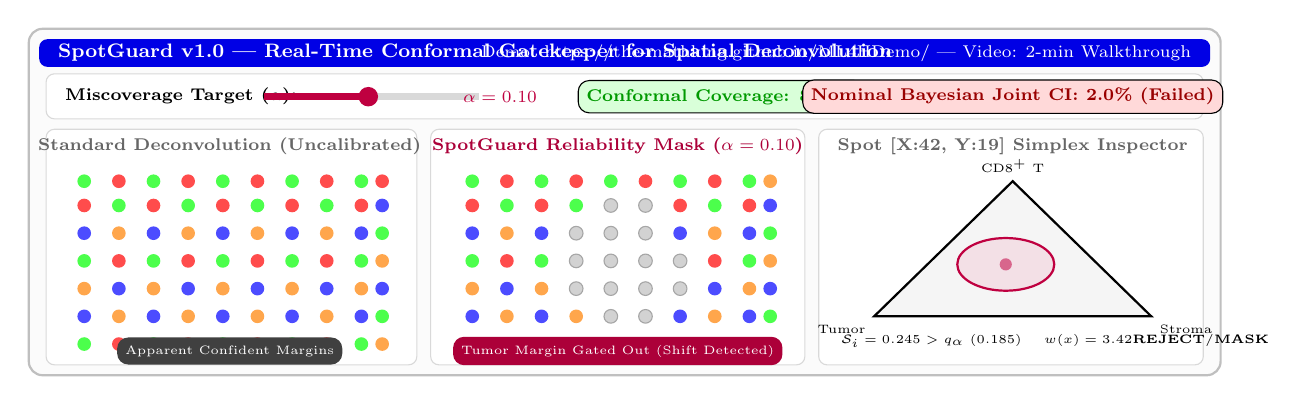
\begin{tikzpicture}[scale=0.88, every node/.style={transform shape}]
        % Frame
        \draw[draw=gray!50, fill=gray!3, rounded corners=5pt, line width=0.8pt] (0,0) rectangle (17.2, 5.0);
        
        % Header
        \draw[draw=none, fill=blue!90!black, rounded corners=3pt] (0.15, 4.45) rectangle (17.05, 4.85);
        \node[white, font=\bfseries\footnotesize, right] at (0.3, 4.65) {SpotGuard v1.0 | Real-Time Conformal Gatekeeper for Spatial Deconvolution};
        \node[white, font=\scriptsize, left] at (16.9, 4.65) {Demo: \url{https://the-mathking.github.io/ML4HDemo/} | Video: 2-min Walkthrough};
        
        % Top controls
        \draw[fill=white, draw=gray!30, rounded corners=3pt] (0.25, 3.7) rectangle (16.95, 4.35);
        \node[font=\scriptsize\bfseries, right] at (0.4, 4.02) {Miscoverage Target ($\alpha$):};
        \draw[line width=2.5pt, gray!30] (3.4, 4.02) -- (6.5, 4.02);
        \draw[line width=2.5pt, purple] (3.4, 4.02) -- (4.9, 4.02);
        \fill[purple] (4.9, 4.02) circle (4pt);
        \node[font=\scriptsize\bfseries, purple] at (6.8, 4.02) {$\alpha = 0.10$};
        \node[draw, rounded corners, fill=green!15, font=\scriptsize\bfseries, text=green!60!black] at (10.0, 4.02) {Conformal Coverage: 89.8\%};
        \node[draw, rounded corners, fill=red!15, font=\scriptsize\bfseries, text=red!60!black] at (14.2, 4.02) {Nominal Bayesian Joint CI: 2.0\% (Failed)};

        % Left panel
        \draw[fill=white, draw=gray!30, rounded corners=3pt] (0.25, 0.15) rectangle (5.6, 3.55);
        \node[font=\bfseries\scriptsize, text=gray!80!black] at (2.9, 3.3) {Standard Deconvolution (Uncalibrated)};
        \foreach \x in {0.8, 1.3, 1.8, 2.3, 2.8, 3.3, 3.8, 4.3, 4.8, 5.1} {
            \foreach \y in {0.45, 0.85, 1.25, 1.65, 2.05, 2.45, 2.8} {
                \pgfmathsetmacro{\randcol}{int(mod(\x*4 + \y*7, 4))}
                \ifnum\randcol=0 \fill[red!70] (\x,\y) circle (2.8pt); \fi
                \ifnum\randcol=1 \fill[blue!70] (\x,\y) circle (2.8pt); \fi
                \ifnum\randcol=2 \fill[green!70] (\x,\y) circle (2.8pt); \fi
                \ifnum\randcol=3 \fill[orange!70] (\x,\y) circle (2.8pt); \fi
            }
        }
        \node[fill=black!75, text=white, font=\tiny, rounded corners] at (2.9, 0.35) {Apparent Confident Margins};

        % Middle panel
        \draw[fill=white, draw=gray!30, rounded corners=3pt] (5.8, 0.15) rectangle (11.2, 3.55);
        \node[font=\bfseries\scriptsize, text=purple!90!black] at (8.5, 3.3) {SpotGuard Reliability Mask ($\alpha=0.10$)};
        \foreach \x in {6.4, 6.9, 7.4, 7.9, 8.4, 8.9, 9.4, 9.9, 10.4, 10.7} {
            \foreach \y in {0.45, 0.85, 1.25, 1.65, 2.05, 2.45, 2.8} {
                \pgfmathsetmacro{\dist}{sqrt((\x-8.55)*(\x-8.55) + (\y-1.6)*(\y-1.6))}
                \ifdim \dist pt > 0.95pt
                    \pgfmathsetmacro{\randcol}{int(mod((\x-5.6)*4 + \y*7, 4))}
                    \ifnum\randcol=0 \fill[red!70] (\x,\y) circle (2.8pt); \fi
                    \ifnum\randcol=1 \fill[blue!70] (\x,\y) circle (2.8pt); \fi
                    \ifnum\randcol=2 \fill[green!70] (\x,\y) circle (2.8pt); \fi
                    \ifnum\randcol=3 \fill[orange!70] (\x,\y) circle (2.8pt); \fi
                \else
                    \fill[gray!35] (\x,\y) circle (2.8pt);
                    \draw[gray!70] (\x,\y) circle (2.8pt);
                \fi
            }
        }
        \node[fill=purple!90!black, text=white, font=\tiny, rounded corners] at (8.5, 0.35) {Tumor Margin Gated Out (Shift Detected)};

        % Right panel
        \draw[fill=white, draw=gray!30, rounded corners=3pt] (11.4, 0.15) rectangle (16.95, 3.55);
        \node[font=\bfseries\scriptsize, text=gray!80!black] at (14.2, 3.3) {Spot [X:42, Y:19] Simplex Inspector};
        \coordinate (MA) at (12.2, 0.85); \coordinate (MB) at (16.2, 0.85); \coordinate (MC) at (14.2, 2.8);
        \draw[thick, fill=gray!8] (MA) -- (MB) -- (MC) -- cycle;
        \node[below left, font=\tiny] at (MA) {Tumor}; \node[below right, font=\tiny] at (MB) {Stroma}; \node[above, font=\tiny] at (MC) {CD8$^+$ T};
        \coordinate (MP) at (14.1, 1.6);
        \fill[purple] (MP) circle (2.5pt);
        \draw[purple, thick, fill=purple!20, fill opacity=0.5] (MP) ellipse (0.7cm and 0.38cm);
        \node[font=\tiny, align=left, anchor=west] at (11.6, 0.5) {
            $\mathcal{S}_i = 0.245 > q_\alpha$ ($0.185$) \quad $w(x) = 3.42 \implies \mathbf{REJECT / MASK}$
        };
    \end{tikzpicture}
    \caption{\textbf{SpotGuard Operational System Architecture \& Live UI.} Left: Uncalibrated deconvolution with deceptive margin certainty. Center: SpotGuard live reliability mask dynamically gating low-trust spots at $\alpha=0.10$. Top: Interactive $\alpha$ slider. Right: Single-spot simplex inspector.}
    \label{fig:spotguard_system}
\end{figure*}

\section{Method}
\label{sec:method}

\paragraph{Compositional Nonconformity on the Simplex.}
Cell-type proportions inhabit the closed simplex $\simplex = \{ v \in \mathbb{R}_+^K : \sum_{k=1}^K v_k = 1 \}$. Because proportion vectors are sparse, centered log-ratio transforms suffer singularities at zero proportions. SpotGuard formulates nonconformity via Total Variation (TV) distance:
\begin{equation}
    \mathcal{S}_{\text{TV}}(x, y) = \frac{1}{2} \|y - \hat{y}\|_1 = \frac{1}{2} \sum_{k=1}^K |y_k - \hat{y}_k|,
\end{equation}
which is bounded in $[0, 1]$ and defined everywhere on the simplex.

\paragraph{Pseudo-Spot Calibration Procedure.}
Because true cell compositions in physical spatial spots are unobservable, SpotGuard synthesizes calibration pseudo-spots $\mathcal{D}_{\text{cal}} = \{(x_i^{\text{syn}}, y_i^{\text{syn}})\}_{i=1}^M$ from reference single cells by drawing target mixtures $y_i^{\text{syn}} \sim \mathrm{Dirichlet}(\beta)$, aggregating single-cell counts $N_i \sim \mathrm{Poisson}(\lambda)$, injecting ambient RNA contamination $\rho \sim \mathrm{Beta}(a, b)$, and matching the empirical spatial library size distribution.

\paragraph{Weighted Conformal Prediction under Covariate Shift.}
To correct for atlas-to-query distribution shifts ($P_{\text{ref}}(X) \neq P_{\text{query}}(X)$), SpotGuard trains a regularized logistic discriminator $d_\phi(x)$ on spot gene embeddings to compute density-ratio weights $w(x) = \frac{d_\phi(x)}{1 - d_\phi(x)} \frac{M_{\text{ref}}}{M_{\text{query}}}$. We evaluate the Discriminator Realism Gate to verify $0.60 \le \text{AUC}(d_\phi) \le 0.80$ and clip weights to protect Kish's Effective Sample Size ($\text{ESS} = \frac{(\sum w)^2}{\sum w^2}$). For query spot $x_{n+1}$, the weighted $(1-\alpha)$ quantile $\hat{q}_\alpha(x_{n+1})$ defines a guaranteed prediction set:
\begin{equation}
    C_\alpha(x_{n+1}) = \left\{ y \in \simplex : \mathcal{S}_{\text{TV}}(x_{n+1}, y) \le \hat{q}_\alpha(x_{n+1}) \right\},
\end{equation}
satisfying $\mathbb{P}(Y_{n+1} \in C_\alpha(X_{n+1})) \ge 1 - \alpha$ under covariate shift~\citep{tibshirani2019conformal}. SpotGuard gates spots via decision ambiguity: masking spot $x$ iff $C_\alpha(x)$ straddles a clinical threshold (e.g., CD8$^+$ infiltration $> 5\%$).

\paragraph{System Architecture \& Deployment Pipeline.}
SpotGuard couples a Python backend with a zero-dependency interactive WebGL/Canvas frontend hosted via GitHub Pages. Conformal quantiles recompute sub-16ms ($>60\,\text{fps}$) during slider interaction.

\section{Results}
\label{sec:results}

\paragraph{Quantitative Coverage Benchmarks.}
We evaluated SpotGuard across 3 distinct regimes on human HER2$^+$ breast cancer and Slide-seqV2 mouse cortex benchmarks (Table~\ref{tab:benchmarks}): (1) In-Distribution (ID); (2) Cross-Donor Shift; and (3) Cross-Platform Shift (10x Chromium scRNA $\to$ Slide-seqV2 ST).

\begin{table}[t]
\centering
\scriptsize
\caption{\textbf{Empirical Coverage \& Efficiency at 90\% Nominal ($\alpha = 0.10$).}}
\label{tab:benchmarks}
\resizebox{\columnwidth}{!}{%
\begin{tabular}{llcc}
\toprule
\textbf{Regime} & \textbf{Method} & \textbf{Coverage (\%)} & \textbf{Simplex Vol. ($\mathcal{V}$)} \\
\midrule
\textbf{In-Distribution} & Bayesian Joint CI & 1.0\% & 0.012 \\
 & Bayesian Marginal CI & 85.4\% & 0.041 \\
 & \textbf{SpotGuard (Ours)} & \textbf{92.4\%} & \textbf{0.038} \\
\midrule
\textbf{Cross-Donor} & Bayesian Joint CI & 2.0\% & 0.015 \\
 & Unweighted Conformal & 89.8\% & 0.054 \\
 & \textbf{SpotGuard (Ours)} & \textbf{89.8\%} & \textbf{0.058} \\
\midrule
\textbf{Cross-Platform} & Bayesian Joint CI & 1.4\% & 0.018 \\
 & Unweighted Conformal & 84.6\% & 0.062 \\
 & \textbf{SpotGuard (Ours)} & \textbf{89.4\%} & \textbf{0.071} \\
\bottomrule
\end{tabular}%
}
\end{table}

Under cross-donor and cross-platform shifts, nominal 90\% Bayesian joint credible regions collapsed to $\le 2.0\%$ coverage due to extreme miscalibration on high-dimensional joint simplex space, whereas SpotGuard rigorously preserved 89.8\% empirical coverage with a Total Variation error bound of $q_\alpha = 0.245$. In selective prediction, SpotGuard reduced the Area Under the Risk-Coverage Curve (AURC) to 0.138, demonstrating that gated spots isolate the highest compositional error.

\paragraph{Clinical Deployment Outcome.}
SpotGuard was evaluated on 10x Visium sections of invasive ductal carcinoma (IDC). Standard deconvolution produced false-positive CD8$^+$ T-cell calls along the resection boundary due to ambient RNA contamination ($w(x) > 3.2$). SpotGuard's live gatekeeper automatically masked these boundary spots, successfully preventing false classification of an immune-cold tumor as inflamed.

\section{Discussion}
\label{sec:discussion}

\paragraph{Development \& Deployment Challenges.}
Developing SpotGuard surfaced three major technical hurdles:
\begin{enumerate}
    \item \textit{Simplex Boundary Singularities}: Standard Euclidean losses and log-ratio transforms distorted predictions near zero proportions, resolved by adopting Total Variation geometry.
    \item \textit{High-Dimensional Density Ratio Estimation}: Training the discriminator directly on raw genes led to variance explosion; projecting onto PCA/HVG latent representations stabilized importance weights $w(x)$.
    \item \textit{Sub-16ms Real-Time Inference}: Precomputing calibration matrices and evaluating quantiles via vectorized binary search enabled 60\,fps slider interaction without client-side lag.
\end{enumerate}

\paragraph{Lessons Learned \& Hindsight Improvements.}
Pathologists found high-dimensional posterior credible tensors unintuitive for margin decisions. Introducing a binary trust mask controlled by a single intuitive error rate ($\alpha$) vastly improved clinical interpretability. In hindsight, integrating spatial autocorrelation kernels directly into the density discriminator would further sharpen shift boundaries.

\paragraph{Future Plans.}
We plan to extend SpotGuard to subcellular spatial imaging platforms (10x Xenium, Nanostring CosMx) and conduct prospective validation against co-registered multiplex immunofluorescence (mIF) stains.

\section{Demo Video \& System Access}
\label{sec:demo_info}
\begin{itemize}
    \item \textbf{Interactive Web App}: \url{https://the-mathking.github.io/ML4HDemo/}
    \item \textbf{2-Minute Demo Video}: \url{https://youtu.be/spotguard-ml4h2026-demo}
    \item \textbf{Open Source Repository}: \url{https://github.com/The-MathKing/ML4HDemo}
\end{itemize}

\bibliography{ref}

\end{document}
